\section{Energiflöde genom fönster}

Vid beräkning av det totala effektflödet genom fönster måste hänsyn tas till minst tre olika typer av källor – konduktion, solstrålning och långvågigstrålning i form av svartkroppstrålning både från omgivningen och från rummets interiör. Här beskrivs vilka resultat som givits vid beräkningar enligt metoderna i föregående kapitel, och börjar med den största källan till värmeflöden, nämligen direkt solstrålning genom fönster. Därefter presenteras resultaten av beräkningarna på långvågsstrålning respektive värmeledning.

\subsection{Direkt solstrålning}
%Skapat med sunfigurestest
I figur~\ref{fig:sun0415and1231} ses de relevanta vinklar som bildas av solens position den 15 april 2011 (heldragna linjer), samt den 31 december 2011 (streckade linjer), beräknat med funktionen sunposition i appendix \ref{app:sunposition}. Den röda linjen visar solens höjd över horisonten medan den gröna indikerar solens azimuthala vinkel, det vill säga vinkel i sidled från en referenspunkt, här tagen till ostlig riktning och medsols. Slutligen representerar den blå linjen i figuren solens vinkel relativt en vertikal ytas normal (då denna pekar i horisontell sydlig riktning) och kan användas för att uppskatta effekten som solinstrålning bidrar till.

\begin{figure}[hpbt]
\centering
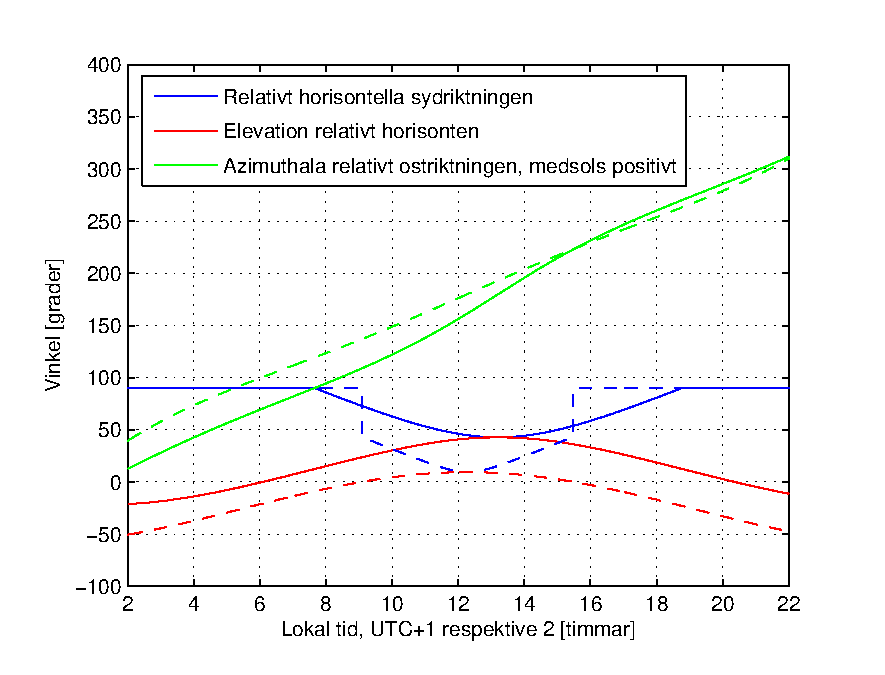
\includegraphics[scale=0.7]{images/sun0415and1231.eps}
\caption{\label{fig:sun0415and1231} Beräknade vinklar vid Walleriusgatan den 15 april 2011 (heldragna linjer, UTC+2) samt den 31 december samma år (streckade linjer, UTC+1).}
\end{figure}

Innan effekten beräknas måste dock ett exempel på solens intensitet över dagen skapas. Detta görs genom sambandet i avsnitt~\ref{sec:sunthroughwindowsmethod}. Longitud och latitud för Walleriusgatan är ungefär 12 $^\circ$E respektive 57,7 $^\circ$N medan jordens medelradie är ungefär $\unit[6,731\cdot 10^{6}]{m}$ \cite{physicshandbook}. Den beräknade intensiteten, som kan ses som de blå linjerna i figur~\ref{fig:effekt0415and1231}, medför att effektflödet genom fönster kan beräknas.

\begin{figure}[hpbt]
\centering
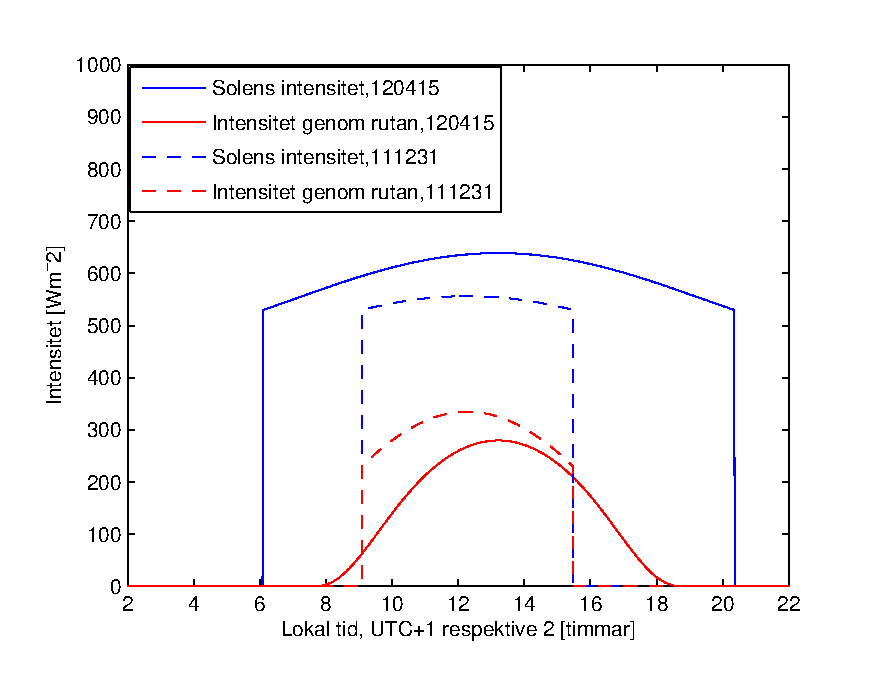
\includegraphics[scale=0.7]{images/effekt0415and1231.eps}
\caption{\label{fig:effekt0415and1231} Beräknad effekt genom ett fönster, vars normal pekar 38$^{\circ}$ öster om horisontella sydriktningen den 15 april 2011 samt den 31 december samma år. Solens intensitet vid marknivå varierar under dagen enligt de blå kurvorna, resulterande i ett flöde genom fönstrena som följer de röda kurvorna. Notera att ingen hänsyn har tagits till skuggor eller persienner och dylikt.}
\end{figure}

Konstanterna $q$ och $p$ i ekvationen för g-värdet, \ref{eq:radiationwindowstheory:gvalue}, sätts till 4 respektive 3, eftersom fönstren i den avsedda byggnaden är av typ treglas utan ytbeläggningar. g-värdet för normal solstrålning, $g_0$, fås från \cite{ASHRAE09} till 0,61. Sydväggens normal pekar åt sydost, med vinkeln 38$^{\circ}$ mot horisontella sydriktningen. Dessa värden på konstanterna ger ett resultat  för den 15 april 2011 och den 31 december samma år, se figur~\ref{fig:effekt0415and1231}.


\subsection{Långvågsstrålning}

Då rummens temperatur skiljer sig från utomhustemperaturen kommer energiflöden via svartkroppsstrålning att uppstå, som det beskrivs i avsnitt~\ref{subsec:IRmethod}. Då temperaturen varierar från $\unit[6]{^{\circ}C}$ klockan 6 på morgonen till $\unit[9]{^{\circ}C}$ klockan 16 på eftermiddagen en aprildag fås en kyleffekt som kan ses i figur~\ref{fig:IRapr}. Då temperaturen istället förändras från $\unit[-11]{^{\circ}C}$ på morgonen till $\unit[-5]{^{\circ}C}$ på eftermiddagen en decemberdag fås istället ett flöde som kan ses i figur~\ref{fig:IRdec}.

\begin{figure}[hpbt]
\centering

\subfloat[\label{fig:IRapr}
Energiflöde från långvågsstrålning en dag i april.]{
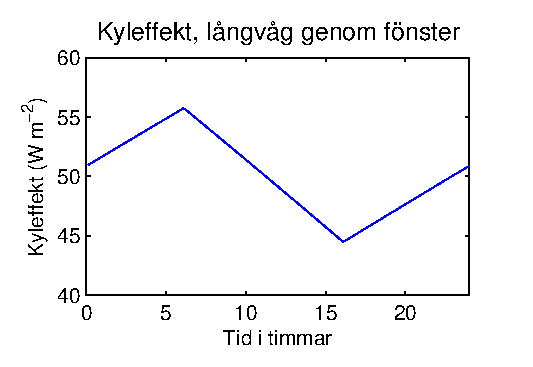
\includegraphics[width=6cm]{images/longwave_apr.eps}}\vspace{1cm}
\subfloat[\label{fig:IRdec}
Energiflöde från långvågsstrålning en dag i december.]{
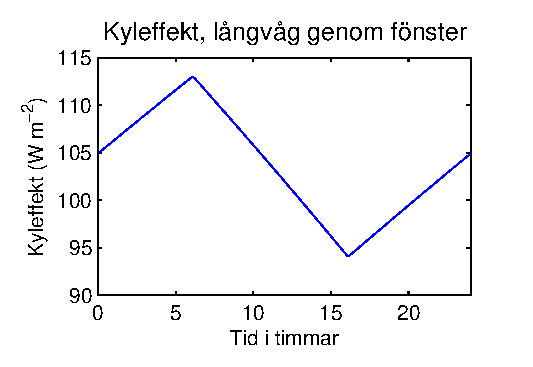
\includegraphics[width=6cm]{images/longwave_dec.eps}
}

\caption{\label{fig:IRwindows} Energiflöden ut genom fönster på grund av långvågsstrålning en dag i mitten av april och den sista december.
Utomhustemperaturen varierar mellan $\unit[6]{^\circ C}$ på natten och $\unit[9]{^\circ C}$ på dagen respektive $\unit[-11]{^\circ C}$ på natten och $\unit[-5]{^\circ C}$ på dagen. Inomhustemperaturen är satt konstant till $\unit[20]{^\circ C}$.}
\end{figure}


\subsection{Värmeledning}

Ytterligare ett värmeflöde genom fönster tillkommer i och med värmeledning. Enligt \cite{petersarneo} har fönstrena ett totalt U-värde $U=\unit[1,0]{Wm^{-2}K^{-1}}$ vilket leder till ett värmeflöde $q_{U}=\unit[T_\text{inne}-T_\text{ute}]{Wm^{-2}}$ där $T_\text{inne}$ sätts konstant till $\unit[20]{^{\circ}C}$ och $T_\text{ute}$ sätts till samma värden som i föregående avsnitt en april- respektive decemberdag. Energiflödena blir alltså $\unit[20]{^{\circ}C}$ minus gällande temperatur som beskrivits i figur~\ref{fig:temperaturedist}.
